\section{The Dataset}

The "Galaxy Zoo" dataset consists of a total \numprint{141553} images. These are split into \numprint{61578} images for training --each with their respective probability distributions for the classifications for each of the inputs-- and \numprint{79975} images for testing.

As a crowd-sourced volunteer effort, images of the dataset were classified across 11 different categories. Each of categories have attributes which volunteers can rank, there are 37 attributes in total. Some categories are dependent on the presence of others, for example number of spiral arms and spiral tightness is dependent on if the galaxy has spiral shape. The votes on these volunteer categorizations are normalized to a floating point number between 0 and 1 inclusive. A number close to 1 indicates many users identified this category for the galaxy image with a high level of confidence, while numbers close to 0 indicate otherwise. These numbers represent the overall morphology of a galaxy in 37 attributes.

Figure \ref{decision-tree} shows how each galaxy's classification is the result of a specific path down the decision tree. The root of the tree consists of more general questions, and as the tree grows, the questions become more specific. The appearance of subsequent questions is dependent upon previous responses. Classifications performed by multiple users for the same galaxy result in multiple paths along the tree which generate probabilities for each question. The classification probability for each node sums up to 1.

Due to these probabilities being tied to each image this is a regression problem rather than a classification problem. Therefore, the task is to determine the degree to which a galaxy has certain attributes and mimic how people would classify the same galaxy.

\begin{figure}[h] \label{decision-tree}
  \centering
  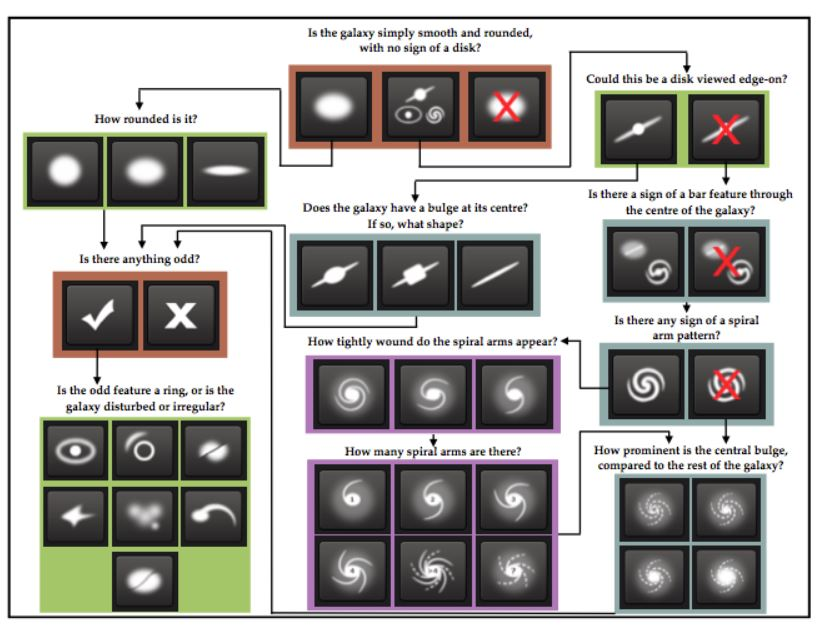
\includegraphics[scale=0.9]{figures/decision-tree.jpg}
  \caption{Flowchart of the classification tasks for the "Galaxy Zoo" dataset. Tasks are color-coded by their relative depths in the decision tree. Tasks outlined in brown are asked for every galaxy. Tasks outlined in green, blue, and purple are (respectively) one, two or three steps below branching points in the decision tree \cite{galaxyzoo2}.}
\end{figure}
